\begin{figure}
    \centering
    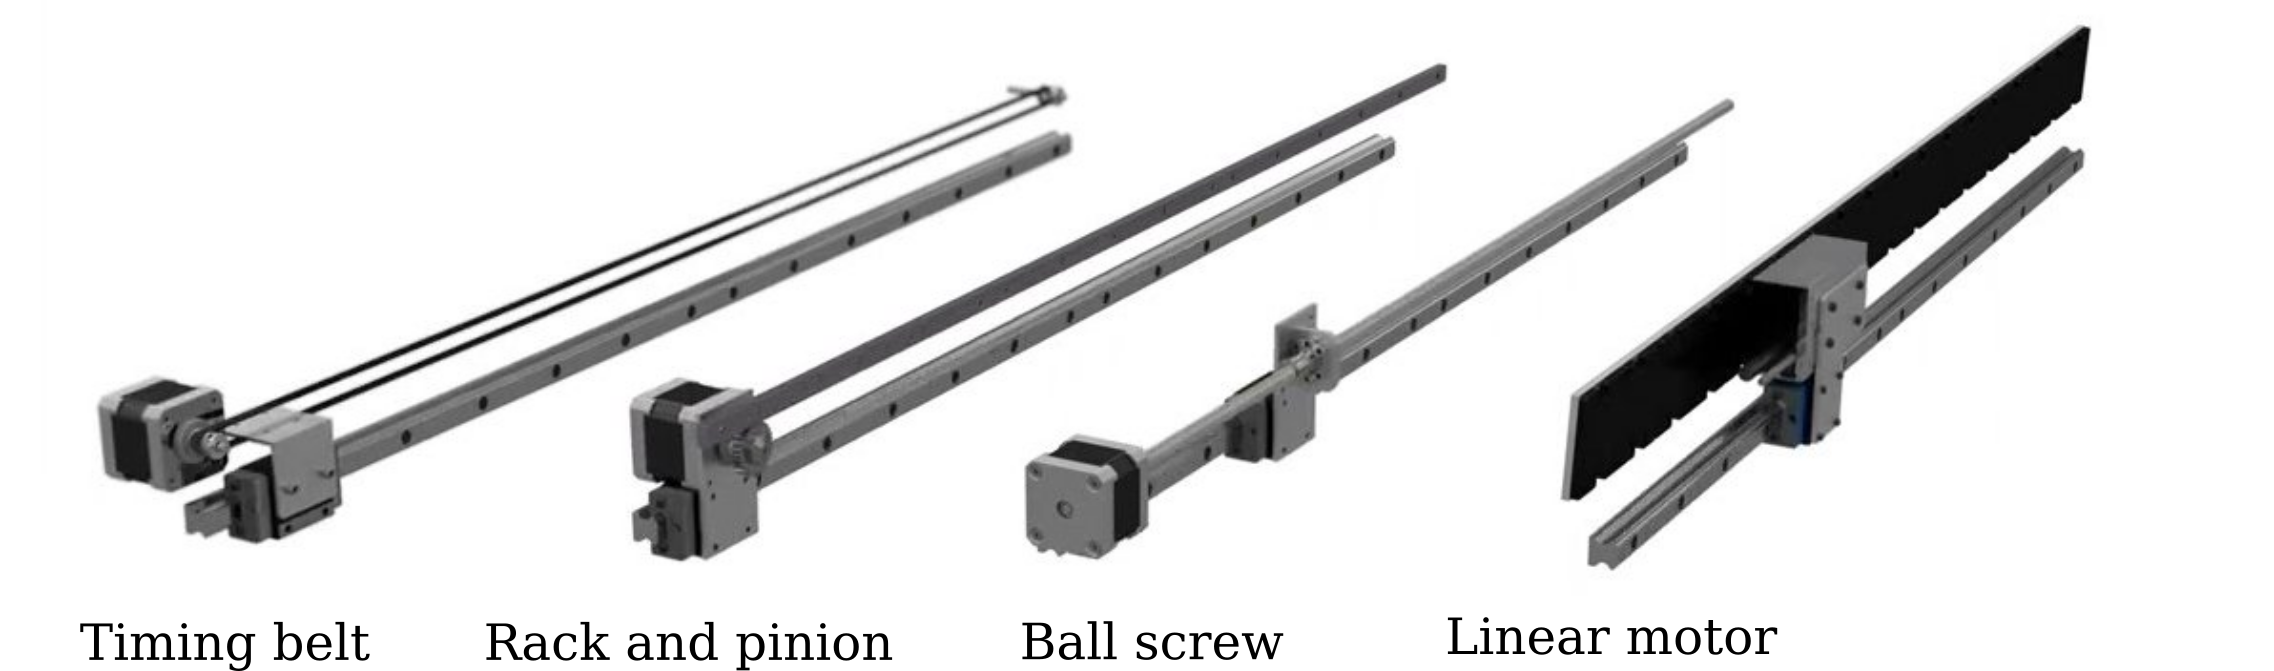
\includegraphics[width=0.9\textwidth]{linear-motion-systems}
    \caption{Linear motion systems}
    \label{fig:linear-motion-systems}
\end{figure}

\begin{figure}
    \centering
    \begin{subfigure}[b]{0.4\textwidth}
        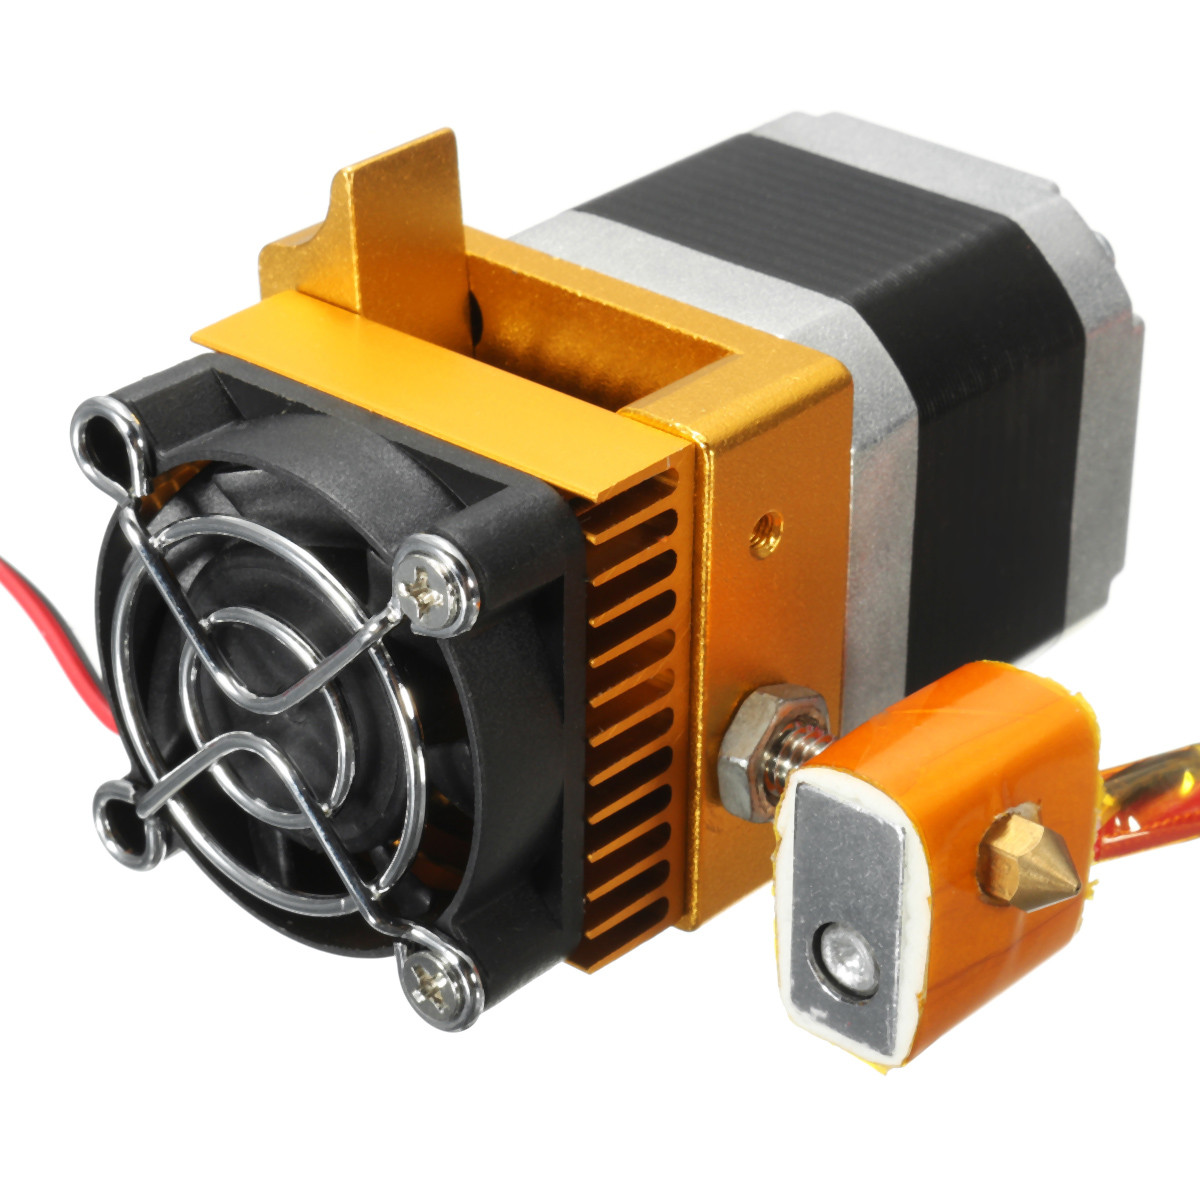
\includegraphics[width=\textwidth]{mk8-extruder}
        \caption{3D printer extruder}
        \label{fig:mk8-extruder}
    \end{subfigure}
    \begin{subfigure}[b]{0.4\textwidth}
        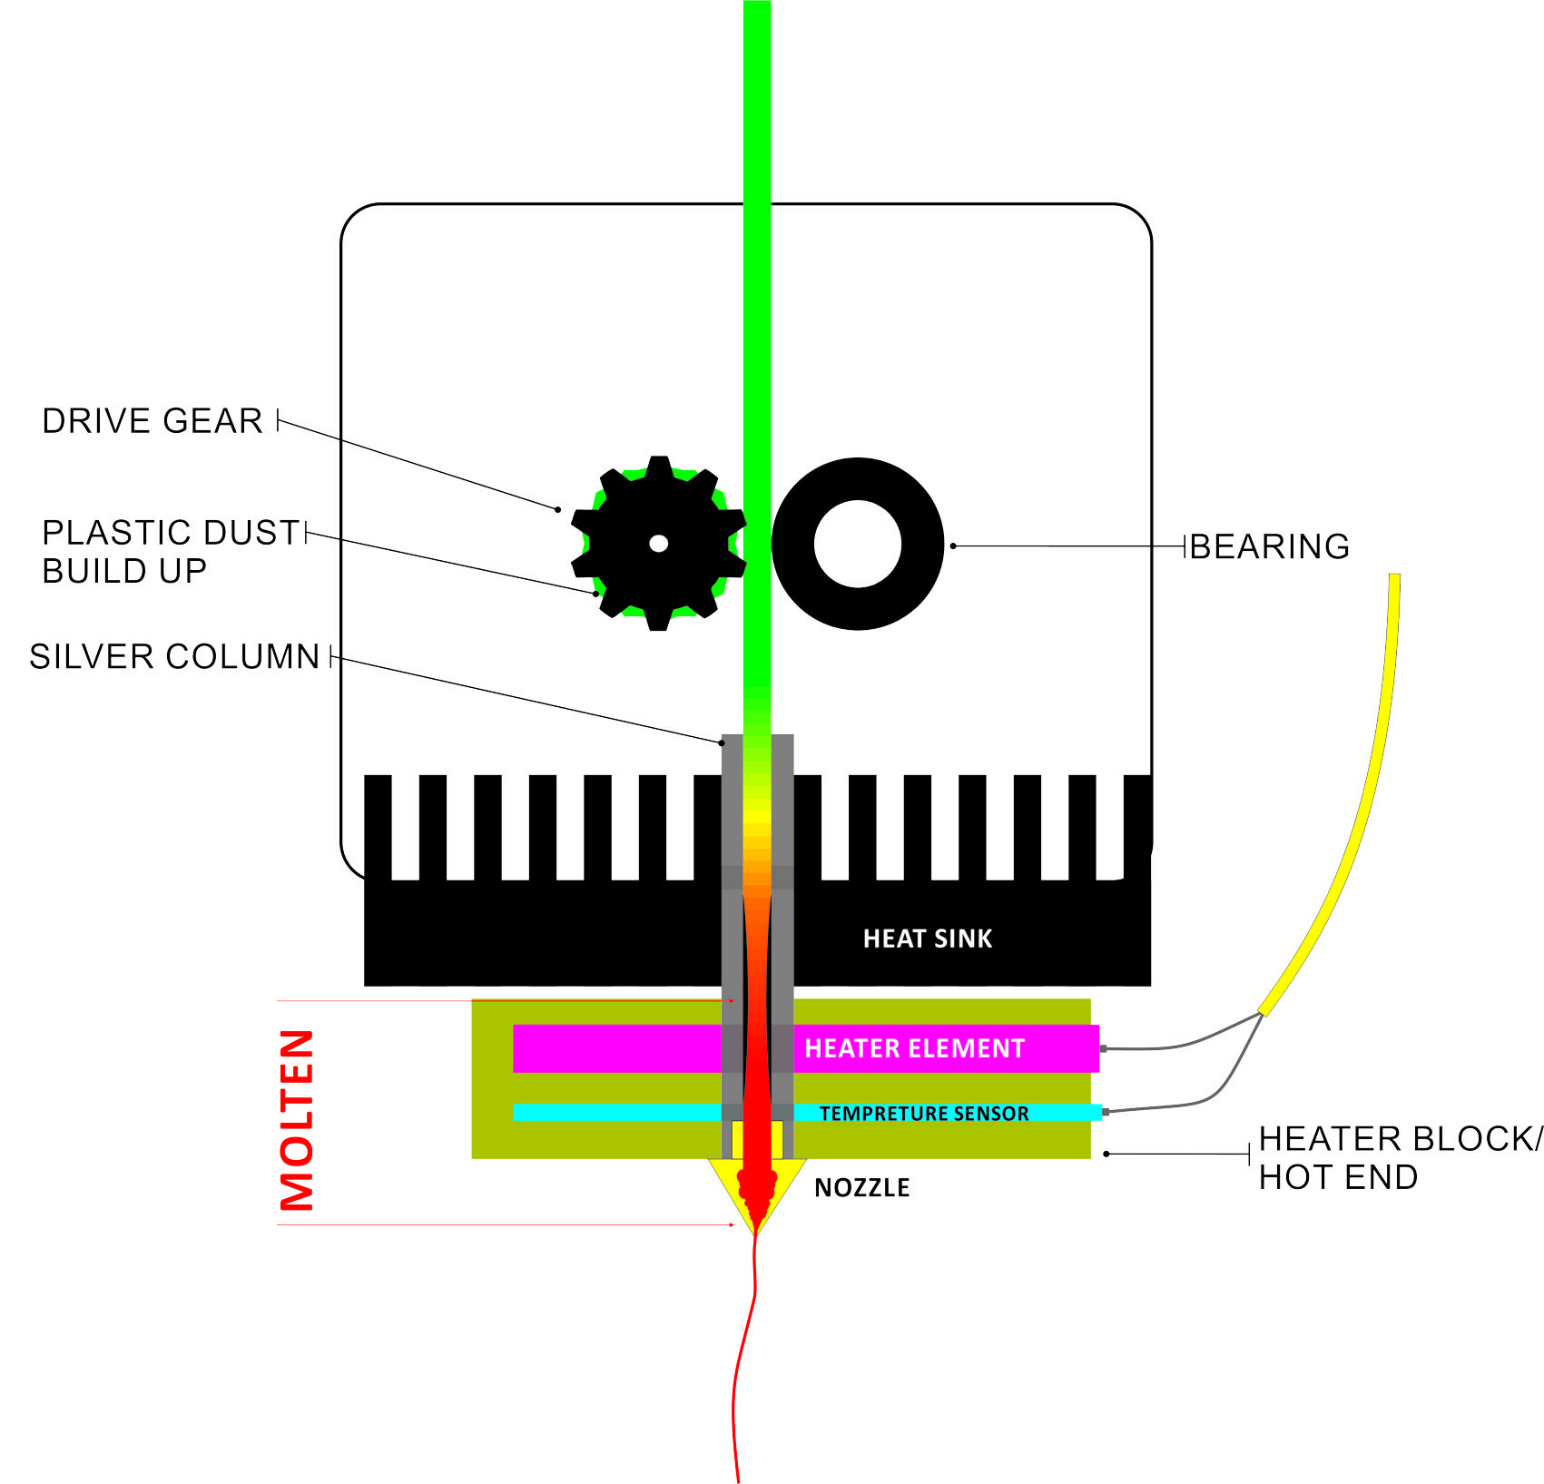
\includegraphics[width=\textwidth]{extruder-function}
        \caption{Functionality of extruder}
        \label{fig:extruder-function}
    \end{subfigure}
    \caption{3D printer extruder}
    \label{fig:extruder}
\end{figure}

\begin{figure}
    \centering
    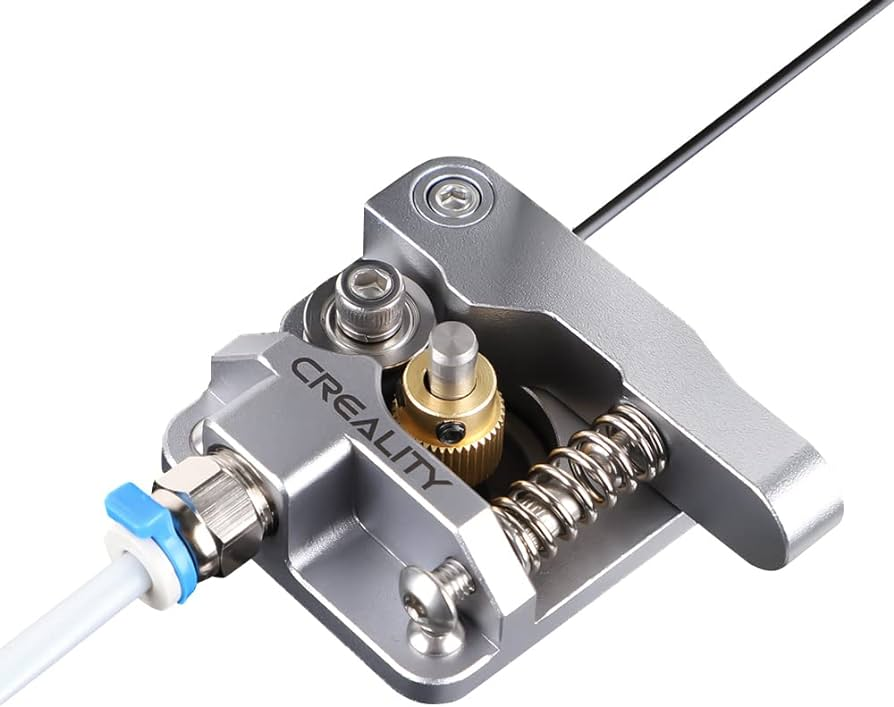
\includegraphics[width=0.5\textwidth]{creality-extruder}
    \caption{Extruder without heater}
    \label{fig:extruder-wo-heater}
\end{figure}


\begin{figure}
    \centering
    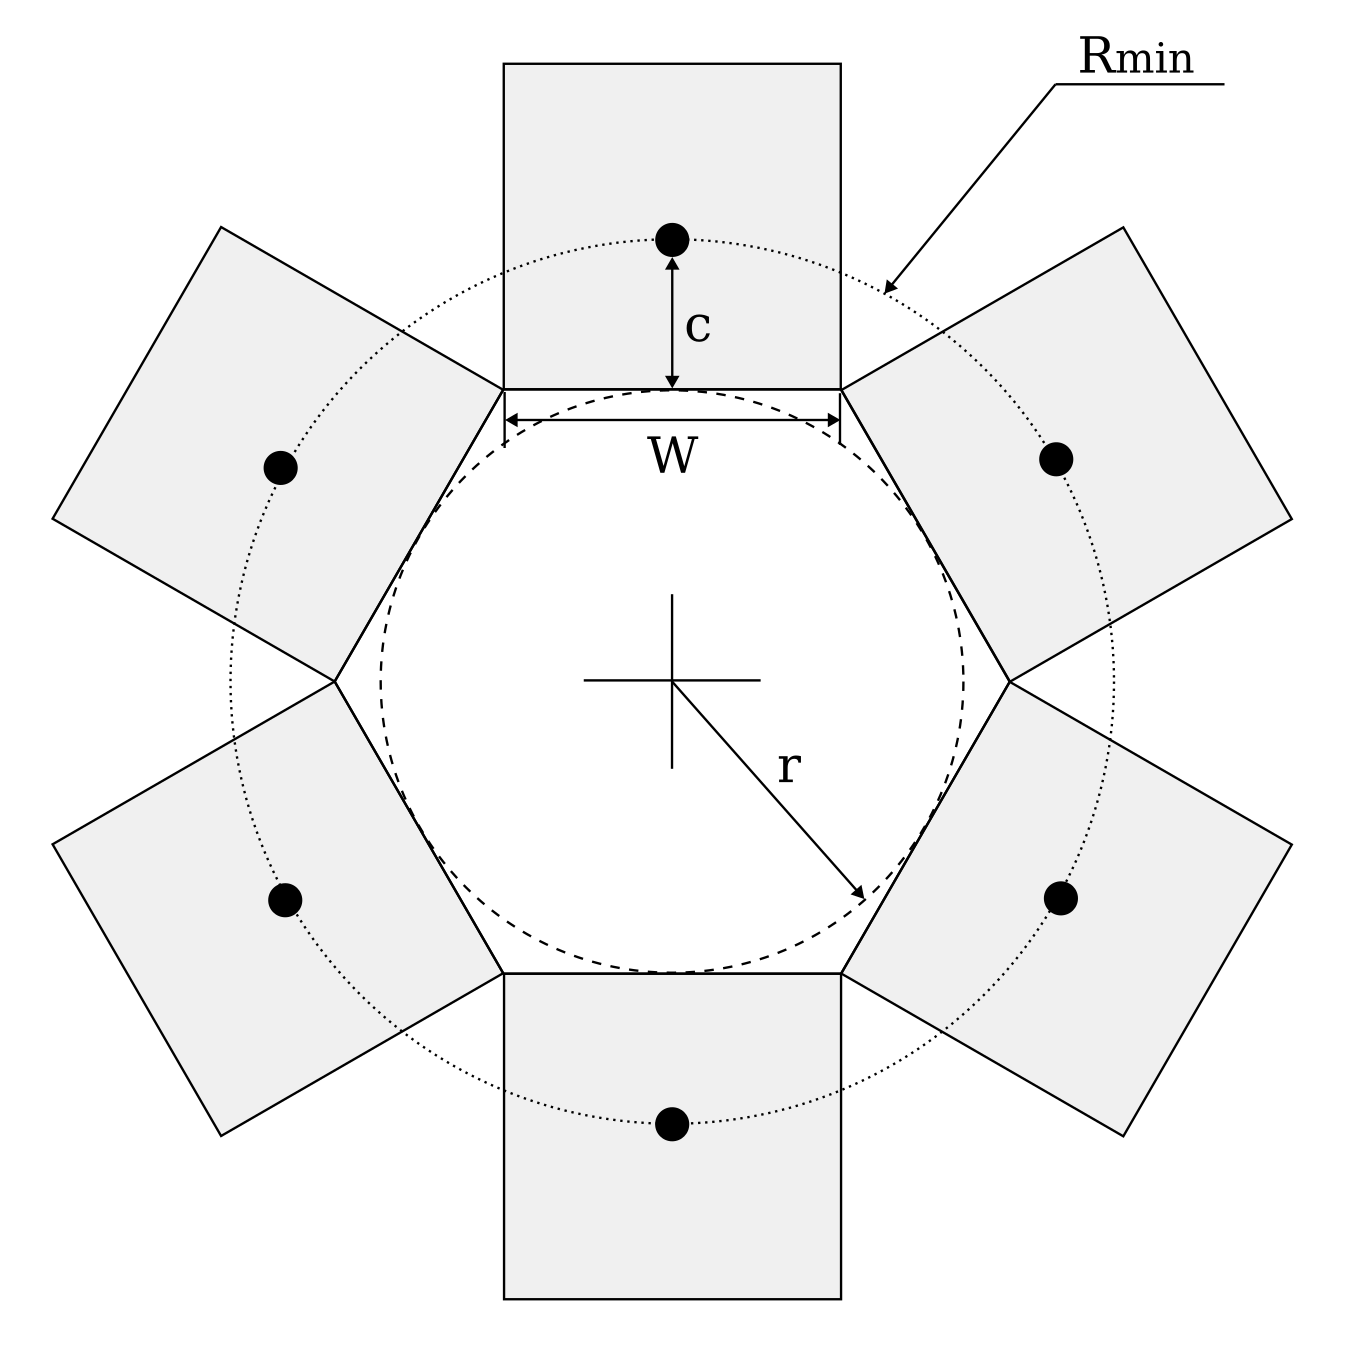
\includegraphics[width=0.7\textwidth]{actuators-arrange}
    \caption{Actuators arrange}
    \label{fig:actuators-arrange}
\end{figure}

$R_{min}=3.5$ cm, $c=0.5$ cm, $W\approx3.5$ cm

Original extruder $W=5.2$ cm, $c=0.7$ cm, $R_{min}=5.2$ cm

\begin{equation}
    r=R_{min}-c
\end{equation}

\begin{equation}
    W=\frac{2}{\sqrt{3}}r
\end{equation}

\begin{equation}
    W=\frac{2}{\sqrt{3}}(R_{min}-c)
\end{equation}

\begin{equation}
    R_{min}=\frac{\sqrt{3}}{2}W+c
\end{equation}


\section{Motor}

\begin{figure}
    \centering
    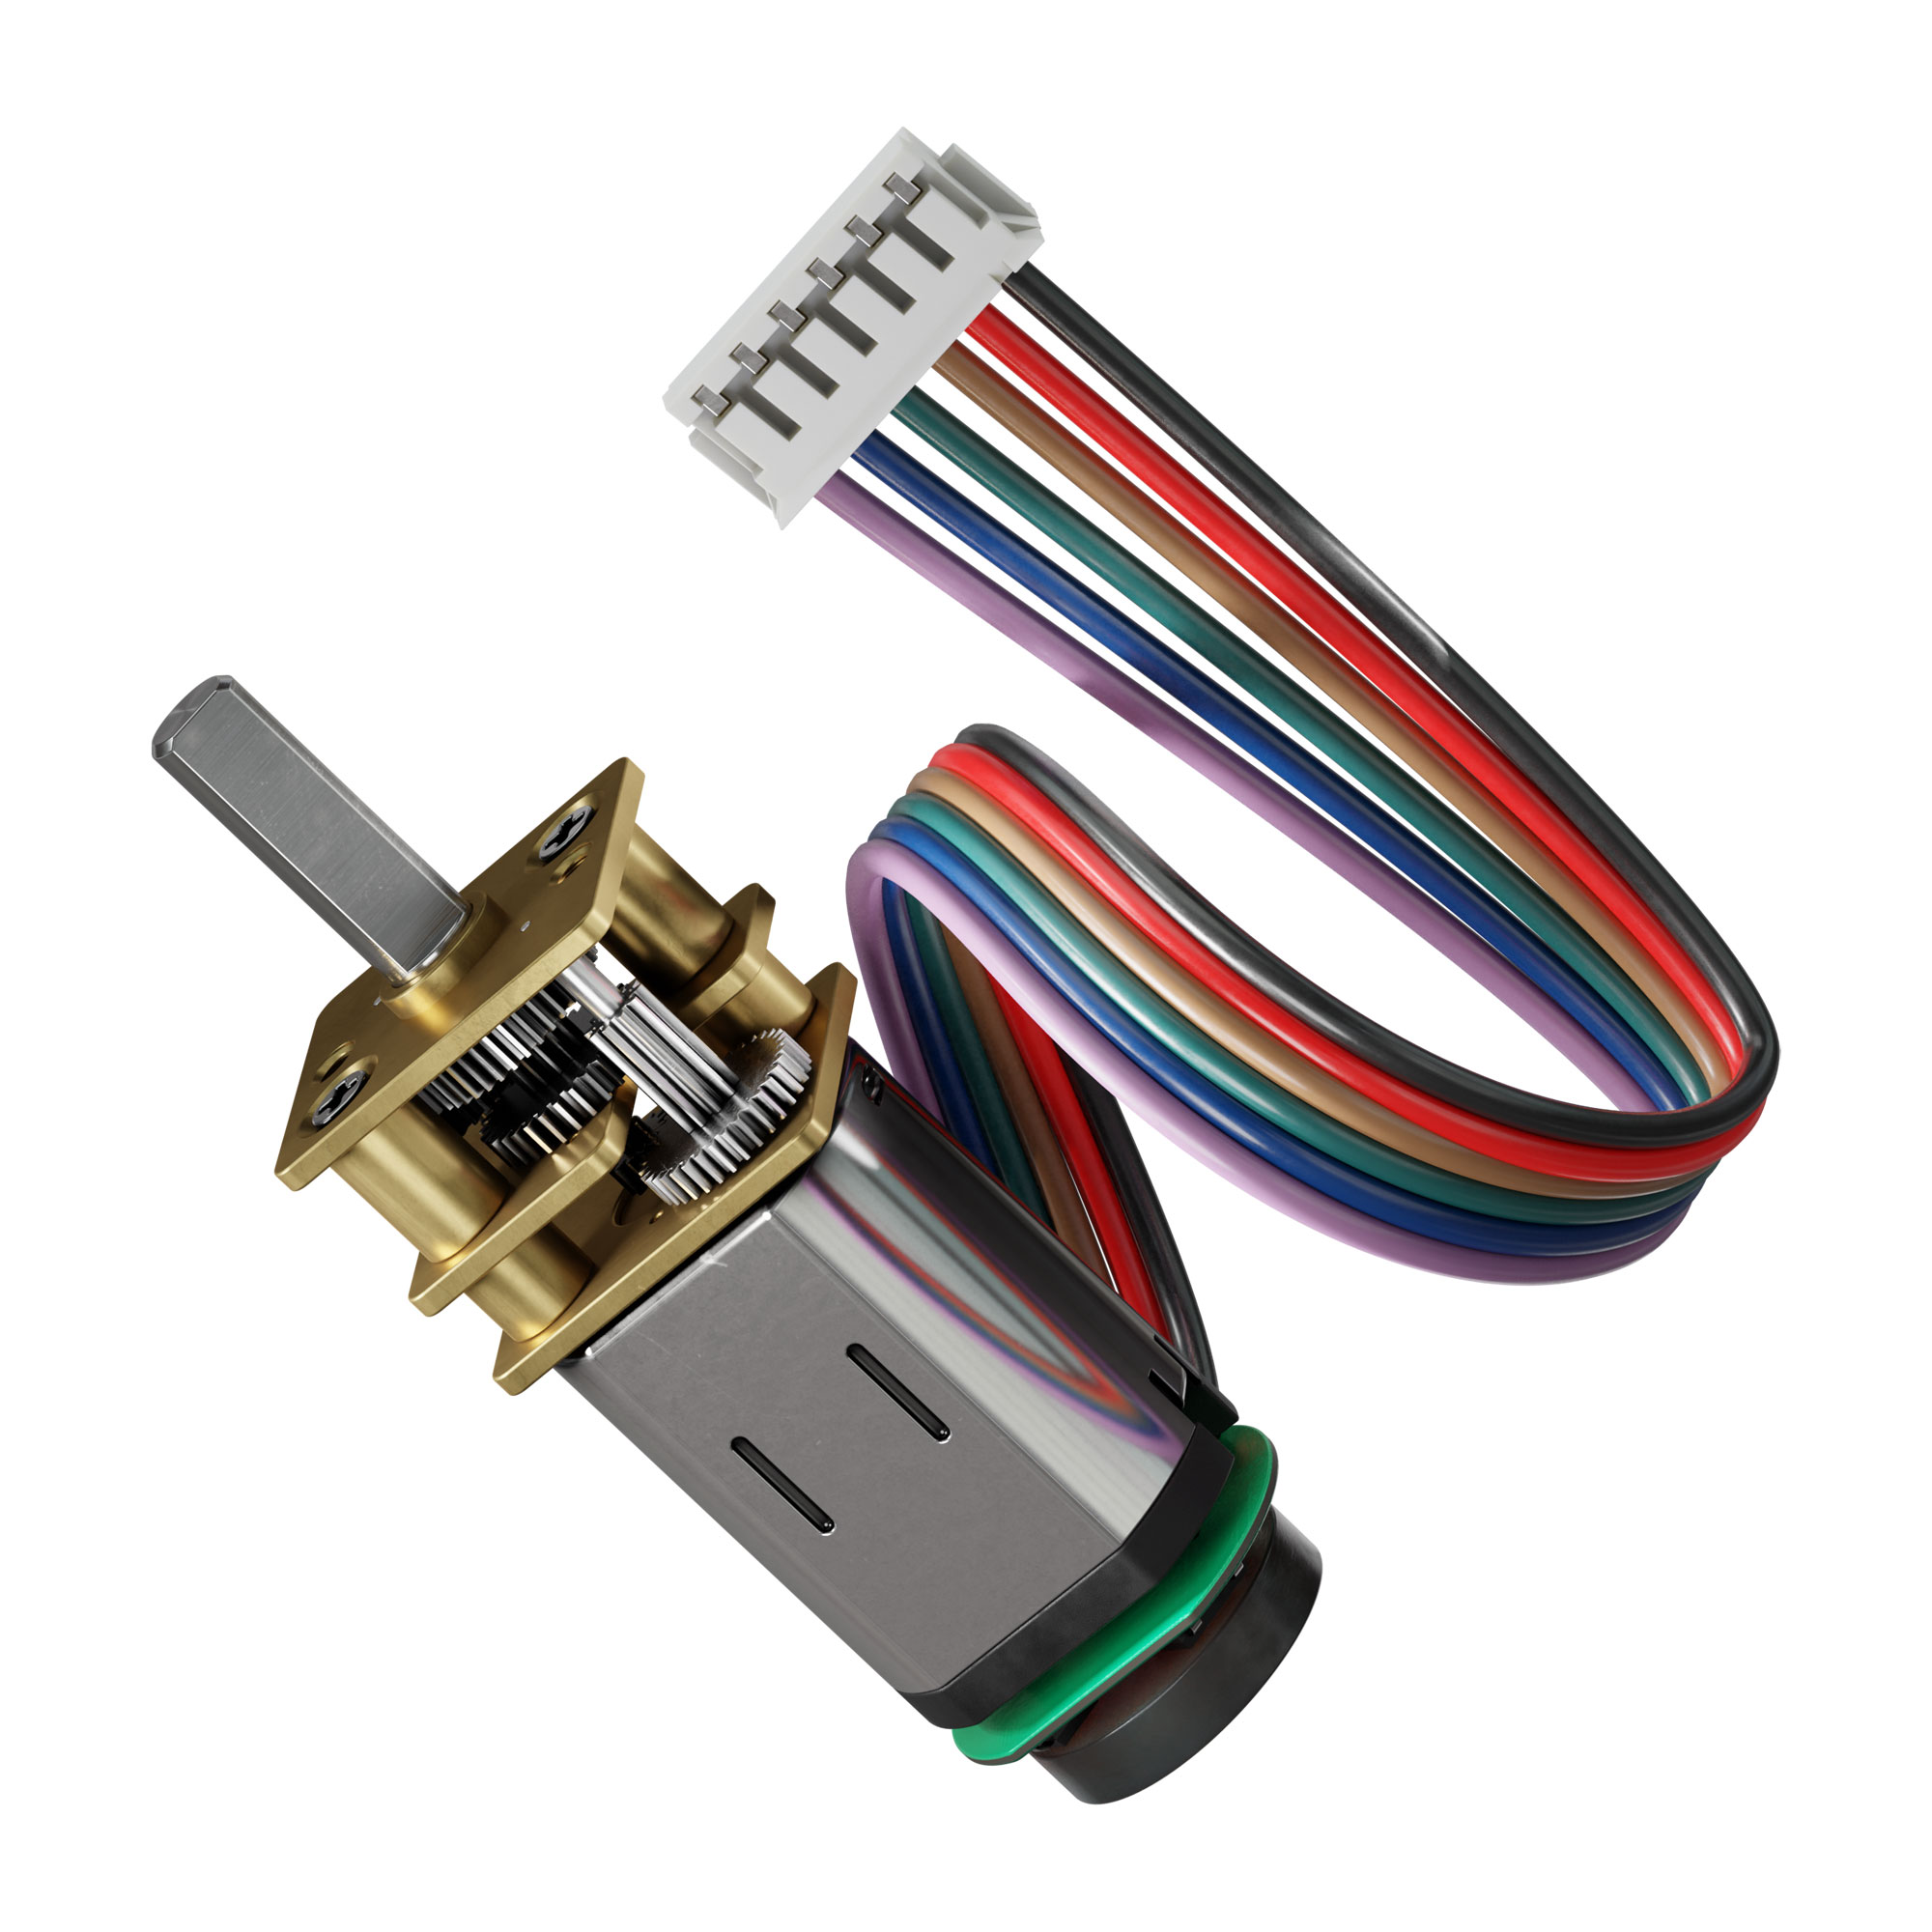
\includegraphics[width=0.45\textwidth]{n20-encoder}
    \caption{Gear motor N20 with encoder}
    \label{fig:n20-encoder}
\end{figure}

\begin{figure}
    \centering
    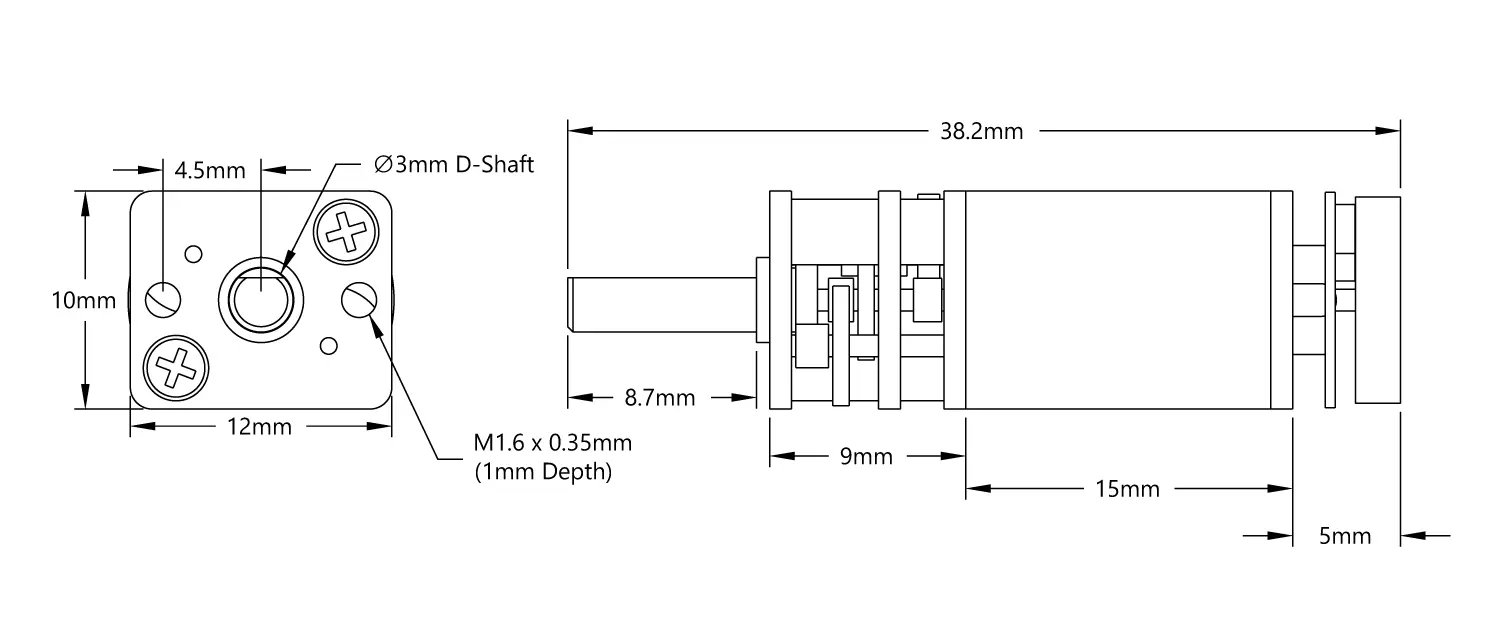
\includegraphics[width=0.9\textwidth]{n20-encoder-dimensions}
    \caption{Dimensions of gear motor N20 with encoder}
    \label{fig:n20-encoder-dimensions}
\end{figure}


\begin{table}[]
    \centering
    \caption{Gear motor specifications}
    \label{tab:motor-specs}
    \begin{tabular}{@{}ll@{}}
    \toprule
    Property                                     & Value                  \\
    \midrule
    Output shaft style                           & D-Shaft                \\
    Voltage range                                & $6-12$V                \\
    Speed (no load @ 6VDC)                       & $70$ rpm               \\
    Rated torque                                 & $0.65$ kg$\cdot$cm            \\
    Stall torque                                 & $4$ kg$\cdot$cm               \\
    Gear ratio                                   & 210:1                  \\
    Weight                                       & $15$g                  \\
    Encoder: cycles per revolution (motor shaft) & 3                      \\
    Encoder sensor type                          & Magnetic (Hall Effect) \\
    Hall response frequency                      & $100$ kHz              \\
    \bottomrule
    \end{tabular}
\end{table}

\section{Components}

\blindtext

\blindtext

\section{Specifications}

\blindtext

\blindtext
